\documentclass{hw_template}

\usepackage{arydshln}

\title{\bfseries Контрольна робота \#1 з Теорії Коливань}
\author{\bfseries Захаров Дмитро}
\date{31 березня, 2025}

\begin{document}

\pagestyle{fancy}

\maketitle

\section{Задача 1}


\begin{problem}
    Тіло маси $m=1.4 \, \text{кг}$ з'єднане за допомогою пружини з жорсткістю
    $k=11340 \, \text{Н}/\text{м}$ з точкою $O$, яка здійснює коливання
    за законом $x_O=a \sin \Omega t$, де $a=0.002 \, \text{м}$, $\Omega=80 \,
    \text{с}^{-1}$. Визначте частоту $\Omega$, при якій настане резонанс.
    Знайдіть амплітуду вимушених коливань системи за заданих значень параметрів.
\end{problem}

\begin{center}
    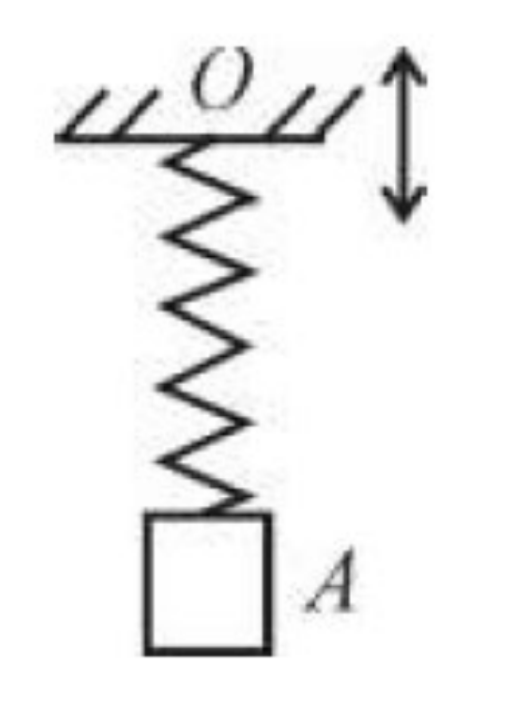
\includegraphics[width=0.2\linewidth]{images/test_1.png}
\end{center}

\textbf{Розв'язання.} Введемо систему координат $O'x$, де $O'$ --- це початкова
точка підвісу, лінія дивиться вниз. Будемо вважати, що відхилення $x_O(t)$
задане у тому самому напрямку. Тоді другий закон Ньютона для тіла маси $m$ можна
записати у вигляді:
\begin{equation*}
    m\ddot{x} = mg - k(x-x_O(t)) = mg - k(x-a\sin\Omega t)
\end{equation*}

Змістимо систему координат на величину $\frac{mg}{k}$: нехай $z := x -
\frac{mg}{k}$. Тоді:
\begin{equation*}
    m\ddot{z} = -kz + ka \sin \Omega t \quad \text{або} \quad \ddot{z} = -\omega^2(z - a \sin \Omega t)
\end{equation*}

Однорідна частина має розв'язок $z=F_1 \cos \omega t + F_2 \sin \omega t$. Неоднорідний 
розв'язок подамо у вигляді $z = F_0 \sin \Omega t$. В такому разі:
\begin{equation*}
    -F_0\Omega^2 \sin \Omega t = -\omega^2(F_0 \sin \Omega t - a \sin \Omega t)
\end{equation*}

Бачимо, що на $\sin \Omega t$ можемо скоротити. Таким чином,
\begin{equation*}
    F_0 = \frac{\omega^2}{\Omega^2}(F_0 - a) \implies F_0 = \frac{\frac{\omega^2}{\Omega^2}}{\frac{\omega^2}{\Omega^2}-1}\cdot a = \frac{a}{1-\frac{\Omega^2}{\omega^2}}
\end{equation*}

Таким чином, загальний розв'язок:
\begin{equation*}
    z(t) = F_1 \cos \omega t + F_2 \sin \omega t + \frac{a}{1-\frac{\Omega^2}{\omega^2}} \sin \Omega t
\end{equation*}

Видно, що резонанс настає за умови $\Omega = \omega$, в іншому випадку амплітуда
вимушених коливань буде $\frac{a}{1-\frac{\Omega^2}{\omega^2}}$.

Підставимо конкретні числа. Маємо частоту $\omega^2 = 11340/1.4 \, \text{с}^{-2}
= 8100 \, \text{с}^{-2}$. Звідси $\omega = 90 \, \text{с}^{-1}$. Це і є частота,
при якій настане резонанс. Проте, за $\Omega=80 \,\text{с}^{-1}$ маємо
$\Omega^2/\omega^2 = 64/81$, тому амплітуда вимушених коливань має вигляд
$\frac{a}{1-64/81} = \frac{81}{17}a \approx 0.0095 \, \text{м}$ або $0.95 \,
\text{см}$. 

\section{Задача 2}

\begin{problem}
    Визначте малі коливання механічної системи з двома ступенями вільності, якщо
функція Лагранжа для неї відома. (Треба визначити власні частоти і форми
коливань)\footnote{Я дещо змінив умову, щоб розмірність Лагранжіана збігалася 
з розмірністю енергії.}
\begin{equation*}
    \mathcal{L}(q,\dot{q}) = \frac{3W_0}{2v_0^2}(\dot{x}^2 + \dot{y}^2 - x^2 - y^2) + \frac{2W_0}{\ell_0^2}xy, \quad q=(x,y),
\end{equation*}
де $W_0,v_0,\ell_0$ --- константи.
\end{problem}

\textbf{Розв'язання.} Знайдемо матриці квадратичних форм потенціальної 
та кінетичної енергій. Трошки перепишемо функцію Лагранжа:
\begin{equation*}
    \mathcal{L}(q,\dot{q}) = \underbrace{\textcolor{blue}{\frac{W_0}{2v_0^2}(3\dot{x}^2 + 3\dot{y}^2)}}_{=\textcolor{blue}{T(\dot{q})}} - \underbrace{\textcolor{red}{\frac{W_0}{2\ell_0^2}\left(3x^2 - 4xy + 3y^2\right)}}_{=\textcolor{red}{V(q)}}
\end{equation*}

Таким чином, маємо вирази для кінетичної та потенціальної енергій:
\begin{align*}
    \textcolor{blue}{T(\dot{q}) = \frac{1}{2}\dot{q}^{\top}A_T\dot{q}}, \quad A_T = \begin{pmatrix}
        3W_0/v_0^2 & 0 \\
        0 & 3W_0/v_0^2
    \end{pmatrix}, \\
    \textcolor{red}{V(q) = \frac{1}{2}q^{\top}A_V q}, \quad A_V = \begin{pmatrix}
        3W_0/\ell_0^2 & -2W_0/\ell_0^2 \\
        -2W_0/\ell_0^2 & 3W_0/\ell_0^2
    \end{pmatrix}
\end{align*}

Для знаходження власних частот та форми коливань, розглянемо допоміжну матрицю
$Q(\omega) = -\omega^2A_T + A_V$. Маємо
\begin{equation*}
    Q(\omega) = \begin{pmatrix}
        3W_0/\ell_0^2 - 3W_0\omega^2/v_0^2 & -2W_0/\ell_0^2 \\
        -2W_0/\ell_0^2 & 3W_0/\ell_0^2 - 3W_0\omega^2/v_0^2
    \end{pmatrix}
\end{equation*}

Власні частоти знаходимо з умови $\det Q(\omega) = 0$: 
\begin{equation*}
    \det Q(\omega) = \left(\frac{3W_0}{\ell_0^2} - \frac{3\omega^2W_0}{v_0^2}\right)^2 - \frac{4W_0^2}{\ell_0^4} = 0 \implies \frac{3W_0}{\ell_0^2} - \frac{3\omega^2W_0}{v_0^2} = \pm \frac{2W_0}{\ell_0^2}
\end{equation*}

Звідси маємо два випадки: $\omega^2=\frac{v_0^2}{3\ell_0^2}$ або $\omega^2 = \frac{5v_0^2}{3\ell_0^2}$. Звідси:
\begin{equation*}
    \omega_1 = \frac{1}{\sqrt{3}}\frac{v_0}{\ell_0}, \quad \omega_2 = \sqrt{\frac{5}{3}} \frac{v_0}{\ell_0}.
\end{equation*}

Для визначення форм коливання, знайдемо власні вектори матриці $Q(\omega)$ для
$\omega=\omega_1$ та $\omega=\omega_2$. Маємо:
\begin{equation*}
    Q(\omega_1) = \begin{pmatrix}
        -2 & -2 \\
        -2 & -2
    \end{pmatrix}\frac{W_0}{\ell_0^2}, \quad Q(\omega_2) = \begin{pmatrix}
        2 & -2 \\
        -2 & 2
    \end{pmatrix}\frac{W_0}{\ell_0^2}
\end{equation*}

Знайдемо власні вектори для обох матриць:
\begin{gather*}
    v_{\omega_1}^{(1)} = \frac{1}{\sqrt{2}}\begin{pmatrix}
        1 \\ 1
    \end{pmatrix}, \quad v_{\omega_1}^{(2)} = \frac{1}{\sqrt{2}}\begin{pmatrix}
        -1 \\ 1
    \end{pmatrix} \\
    v_{\omega_2}^{(1)} = \frac{1}{\sqrt{2}}\begin{pmatrix}
        -1 \\ 1
    \end{pmatrix}, \quad v_{\omega_2}^{(2)} = \frac{1}{\sqrt{2}}\begin{pmatrix}
        1 \\ 1
    \end{pmatrix}
\end{gather*}

Отже видно, що відношення $x_1/x_2$ для першої частоти дорівнює $1$ (себто дві
координати збігаються), а для другої частоти дорівнює $-1$ (тобто вони
протилежні).

\section{Задача 3}

\begin{problem}
    Вантаж на пружині рухається згідно рівнянню:
    \begin{equation*}
        m\ddot{x} + kx = \sum_{i=1}^n f_i \cos \omega_i t
    \end{equation*}
    Визначте закон руху вантажу, якщо в початковий момент часу його переміщення
та швидкість дорівнювали нулю. Зокрема, розгляньте випадок, де права частина має
вигляд $5f_0 \cos \Omega t + 2f_0 \cos 3\Omega t$. Визначте також, за якої умови
виникне резонанс.
\end{problem}

\textbf{Розв'язання.} Розв'язком однорідної частини є $x(t) = A \cos (\omega_0 t + \varphi_0)$, 
де $\omega_0 = \sqrt{k/m}$, а $A$ та $\varphi_0$ --- константи, які
визначаються з початкових умов. 

Для визначення загального розв'язку неоднорідної частини, потрібно знайти $n$
часткових розв'язків для кожного $f_i \cos \omega_i t$. Для цього кожен з
часткових розв'язків будемо шукати у вигляді $\widetilde{x}_i(t) =
\widetilde{a}_i \cos \omega_i t$. Тоді, підставивши у рівняння, отримаємо:
\begin{equation*}
    -m\omega_i^2 \widetilde{a}_i \cos \omega_i t + k\widetilde{a}_i \cos \omega_i t = f_i \cos \omega_i t \implies (-m\omega_i^2 + k)\widetilde{a}_i = f_i
\end{equation*}

Звідси отримуємо амплітуду кожного доданку:
\begin{equation*}
    \widetilde{a}_i = \frac{f_i}{k-m\omega_i^2} = \frac{f_i}{m\left(\frac{k}{m}-\omega_i^2\right)} = \frac{f_i}{m(\omega_0^2-\omega_i^2)} = \frac{1}{1-\frac{\omega_i^2}{\omega_0^2}}\cdot\frac{f_i}{m\omega_0^2}
\end{equation*}

Таким чином, загальний розв'язок:
\begin{equation*}
    x(t) = A \cos (\omega_0 t + \varphi_0) + \sum_{i=1}^n \frac{1}{1-\frac{\omega_i^2}{\omega_0^2}}\cdot\frac{f_i}{m\omega_0^2}\cos \omega_i t
\end{equation*}

Оскільки початкова швидкість нульова, то:
\begin{equation*}
    \dot{x}(t) = -A\omega_0 \sin(\omega_0 t + \varphi_0) - \sum_{i=1}^n \frac{1}{1-\frac{\omega_i^2}{\omega_0^2}}\cdot\frac{f_i\omega_i}{m\omega_0^2}\sin \omega_i t
\end{equation*}

Оскільки $\dot{x}(0) = -A\omega_0 \sin \varphi_0 = 0$, то $\varphi_0=0$. При
умові $x(0)=0$ маємо:
\begin{equation*}
    x(0) = A + \sum_{i=1}^n \frac{1}{1-\frac{\omega_i^2}{\omega_0^2}}\cdot\frac{f_i}{m\omega_0^2} = 0 \implies A = -\sum_{i=1}^n \frac{1}{1-\frac{\omega_i^2}{\omega_0^2}}\cdot\frac{f_i}{m\omega_0^2}
\end{equation*}

Таким чином, маємо:
\begin{equation*}
    \boxed{x(t) = \frac{1}{m\omega_0^2}\sum_{i=1}^n \frac{f_i}{1-\frac{\omega_i^2}{\omega_0^2}}\left(\cos \omega_i t - \cos \omega_0 t\right)}
\end{equation*}

Підставимо конкретні числа. Маємо $f_1=5f_0$, $\omega_1=\Omega$, $f_2=2f_0$, $\omega_2=3\Omega$. Маємо:
\begin{equation*}
    x(t) = \frac{f_0}{m\omega_0^2}\left( \frac{2(\cos 3\Omega t - \cos \omega_0 t)}{1 - \frac{9\Omega^2}{\omega_0^2}} + \frac{5(\cos \Omega t - \cos \omega_0 t)}{1 - \frac{\Omega^2}{\omega_0^2}}\right)
\end{equation*}

Бачимо, що знаменник різко зростає за умови $\omega_0^2=9\Omega^2$ та
$\omega_0^2=\Omega^2$, себто $\omega_0=\Omega$ та $\omega_0=3\Omega$.
Зокрема, це видно на графіку \ref{fig:my_label}.

\begin{figure}
    \centering
    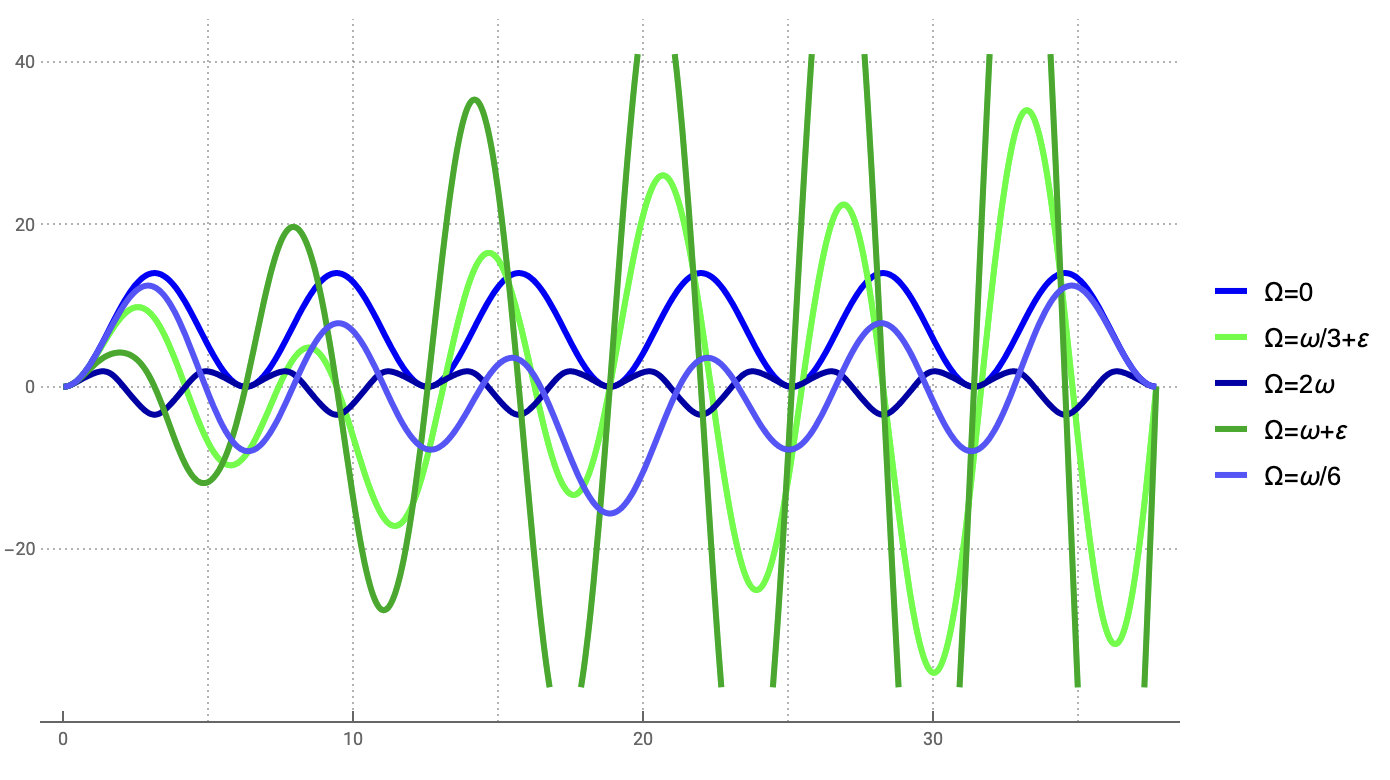
\includegraphics[width=0.8\linewidth]{images/test_1_problem_3.png}
    \caption{Графік $x(t)$ за різних відношень $\Omega/\omega_0$. Видно, що за умови $\Omega/\omega=1/3$ та $\Omega/\omega=1$ виникає резонанс. Зеленим показані коливання, близькі до резонансу, синім --- далеко від резонансу.}
    \label{fig:my_label}
\end{figure}

\end{document}